% Important: If latex complains about unicode characters,
% please use "\usepackage[utf8x]{inputenc}" in your preamble
% You can change the size of the picture by putting it into the construct:
% 1) \resizebox{10cm}{!}{"below picture"} to scale horizontally to 10 cm
% 2) \resizebox{!}{15cm}{"below picture"} to scale vertically to 15 cm
% 3) \resizebox{10cm}{15cm}{"below picture"} a combination of above two
% It is not recomended to use the scale option of the tikzpicture environment.
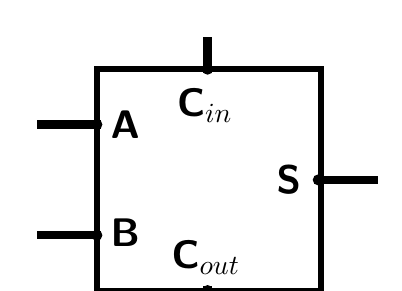
\begin{tikzpicture}[x=1pt,y=-1pt,line cap=rect]
\useasboundingbox (0,0) rectangle (125,85);
\definecolor{custcol_0_0_0}{RGB}{0, 0, 0}
\definecolor{custcol_ff_ff_ff}{RGB}{255, 255, 255}
\draw [line width=3.0pt, custcol_0_0_0 ]  (65.0,95.0) -- (65.0,105.0) ;
\draw [line width=3.0pt, custcol_0_0_0 ]  (65.0,5.0) -- (65.0,15.0) ;
\draw [line width=3.0pt, custcol_0_0_0 ]  (5.0,35.0) -- (25.0,35.0) ;
\draw [line width=3.0pt, custcol_0_0_0 ]  (5.0,75.0) -- (25.0,75.0) ;
\draw [line width=3.0pt, custcol_0_0_0 ]  (105.0,55.0) -- (125.0,55.0) ;
\fontsize{14pt}{14pt}\fontseries{bx}\sffamily\selectfont\node[inner sep=0, outer sep=0, custcol_0_0_0, anchor=base west] at  (52.0,87.0)  {\textbf{C$_{out}$}};
\fontsize{14pt}{14pt}\fontseries{bx}\sffamily\selectfont\node[inner sep=0, outer sep=0, custcol_0_0_0, anchor=base west] at  (90.0,60.0)  {\textbf{S}};
\fontsize{14pt}{14pt}\fontseries{bx}\sffamily\selectfont\node[inner sep=0, outer sep=0, custcol_0_0_0, anchor=base west] at  (30.0,79.0)  {\textbf{B}};
\fontsize{14pt}{14pt}\fontseries{bx}\sffamily\selectfont\node[inner sep=0, outer sep=0, custcol_0_0_0, anchor=base west] at  (30.0,40.0)  {\textbf{A}};
\draw [line width=2.0pt, custcol_0_0_0 ]  (25.0,15.0) -- (105.0,15.0) ;
\draw [line width=2.0pt, custcol_0_0_0 ]  (106.0,15.0) -- (106.0,94.0) ;
\draw [line width=2.0pt, custcol_0_0_0 ]  (106.0,95.0) -- (26.0,95.0) ;
\draw [line width=2.0pt, custcol_0_0_0 ]  (25.0,95.0) -- (25.0,16.0) ;
\fontsize{14pt}{14pt}\fontseries{bx}\sffamily\selectfont\node[inner sep=0, outer sep=0, custcol_0_0_0, anchor=base west] at  (54.0,32.0)  {\textbf{C$_{in}$}};
\fill [line width=1.0pt, custcol_0_0_0]  (25.0,35.0) ellipse (2.0 and 2.0 );
\fill [line width=1.0pt, custcol_0_0_0]  (25.0,75.0) ellipse (2.0 and 2.0 );
\fill [line width=1.0pt, custcol_0_0_0]  (65.0,15.0) ellipse (2.0 and 2.0 );
\fill [line width=1.0pt, custcol_0_0_0]  (65.0,95.0) ellipse (2.0 and 2.0 );
\fill [line width=1.0pt, custcol_0_0_0]  (105.0,55.0) ellipse (2.0 and 2.0 );
\end{tikzpicture}

